% Intestazione
\fancyhead[L]{3 \hspace{0.2cm} Casi d'uso} % Testo a sinistra


\section{Casi d'uso}
\label{sec:casi_uso}

\subsection{Scopo}

Lo scopo di questa sezione è descrivere in maniera dettagliata i casi d’uso individuati dal
gruppo, in riferimento alle funzionalità dell’applicazione.


\subsection{Attori}
\label{sec:attori}

L’applicazione prevede la presenza di sei \emph{Attori}\textsubscript{\textbf{\textit{G}}} principali:

\begin{itemize}
    \item \textbf{Utente}: Persona che utilizza l'applicazione interagendo direttamente con il sistema e avendo accesso a tutte le funzionalità del chatbot.
    \item \textbf{\emph{GitHub}\textsubscript{\textbf{\textit{G}}}}: Piattaforma di gestione del codice sorgente che fornisce i documenti necessari per il modello di question answering. \emph{GitHub} è utilizzato come fonte di dati, mettendo a disposizione documentazione, repository e informazioni sui progetti. Oltre a fornire i documenti, \emph{GitHub} viene utilizzato anche per gestire i task da svolgere, attraverso l'uso delle issue, che il modello può consultare per rispondere alle domande degli utenti relative al codice, ai progetti e alle attività da completare.
    \item \textbf{\emph{Jira}\textsubscript{\textbf{\textit{G}}}}: Piattaforma per la gestione dei progetti e il tracciamento delle attività. Il suo compito è fornire documentazione relativa ai task, alle issue e ai progressi dei progetti. \emph{Jira} viene utilizzato come fonte di dati per il modello di question answering, consentendo al sistema di accedere a informazioni su problemi, progressi e attività legate ai progetti per rispondere alle domande degli utenti.
    \item \textbf{\emph{Confluence}\textsubscript{\textbf{\textit{G}}}}: Piattaforma per la gestione della documentazione collaborativa. \emph{Confluence} offre documenti e altre informazioni condivise tra i membri del team, riguardanti i vari progetti. Viene utilizzata come fonte di dati dal modello di question answering, che sfrutta la documentazione per fornire risposte precise e contestualizzate alle domande degli utenti.
    \item \textbf{\emph{Database vettoriale}\textsubscript{\textbf{\textit{G}}}}: Il database vettoriale è un sistema usato per memorizzare informazioni sotto forma di vettori. È progettato per rendere più semplice e veloce la ricerca semantica, sfruttando algoritmi di intelligenza artificiale e di similarità. Supporta il modello di question answering nell'archiviazione e nel recupero rapido di documenti da GitHub, Jira e Confluence, permettendo al sistema di rispondere in modo efficiente trovando contenuti rilevanti tramite il confronto tra vettori.
    \item \textbf{\emph{Modello di embedding}\textsubscript{\textbf{\textit{G}}}}: Il modello di embedding è un sistema di intelligenza artificiale che trasforma i documenti in vettori numerici. Questo modello è utilizzato per convertire i documenti provenienti da \emph{GitHub}, \emph{Jira} e \emph{Confluence} in vettori, in modo da poterli memorizzare e confrontare in maniera efficiente all'interno del database vettoriale. Il modello di embedding è fondamentale per il funzionamento del sistema, in quanto permette di elaborare e confrontare i dati in modo rapido e preciso.
    \item \textbf{\emph{Scheduler}\textsubscript{\textbf{\textit{G}}}}: Lo \emph{Scheduler} è un sistema che si occupa di pianificare e gestire l'aggiornamento automatico periodico del \emph{database vettoriale}. Lo \emph{Scheduler} è fondamentale per mantenere il database aggiornato e garantire che il sistema abbia sempre a disposizione le informazioni più recenti e precise per rispondere alle domande degli utenti.

\end{itemize}


\subsection{Lista casi d'uso}




% TEMPLATE

\begin{comment}
\hypertarget{UC0}{}
\subsubsection{UC0: \dots}

\begin{figure}[h]
    \centering
    
\includegraphics[width=\textwidth]{placeholder.png}
    \caption{\dots}
\end{figure}

\begin{itemize}
    \item \textbf{Attori principali}: \dots;
    \item \textbf{Precondizioni}: \dots;
    % Oppure, se ci sono più precondizioni:
    \item \textbf{Precondizioni}: 
    \begin{itemize}
        \item \dots;
        \item \dots.
    \end{itemize}
    \item \textbf{Trigger}: \dots;
    \item \textbf{Postcondizioni}: \dots;
    \item \textbf{Scenario principale}:
    \begin{enumerate}
        \item \dots;
        \item \dots.
    \end{enumerate}
    \item \textbf{Sottocasi d'uso}:
    \begin{itemize}
        \item \dots;
        \item \dots.
    \end{itemize}
    \item \textbf{Scenario alternativo}:
    \begin{enumerate}
        \item \dots;
        \item \dots.
    \end{enumerate}
\end{itemize}
\end{comment}




\hypertarget{UC1}{}
\subsubsection{UC1: Inserimento di un'interrogazione in linguaggio naturale}

\begin{figure}[h]
    \centering
    
\includegraphics[width=\textwidth]{placeholder.png}
    \caption{Inserimento di un'interrogazione in linguaggio naturale}
\end{figure}

\begin{itemize}
    \item \textbf{\emph{Attori} principali}: Utente;
    \item \textbf{Precondizioni}: L'utente deve avere accesso all'interfaccia dell'applicazione connessa al database;
    \item \textbf{\emph{Trigger}\textsubscript{\textbf{\textit{G}}}}: L'utente desidera inserire un'interrogazione in linguaggio naturale nella barra di input;
    \item \textbf{Postcondizioni}: L'interrogazione viene inviata e, se valida, genera una risposta adeguata. Se non valida, l'utente riceve un messaggio di errore;
    \item \textbf{\emph{Scenario principale}\textsubscript{\textbf{\textit{G}}}}:
    \begin{enumerate}
        \item L'utente accede all'interfaccia dell'applicazione;
        \item \bulhyperlink{UC1.1}{UC1.1}: L'utente scrive l'interrogazione in linguaggio naturale nella barra di input.
        \item \bulhyperlink{UC1.3}{UC1.3}: Il sistema valida l'interrogazione.
        \item \bulhyperlink{UC1.4}{UC1.4}: Il sistema mostra il messaggio generato nella schermata principale.
    \end{enumerate}
    \item \textbf{\emph{Sottocasi d'uso}\textsubscript{\textbf{\textit{G}}}}:
    \begin{itemize}
        \item \bulhyperlink{UC1.1}{UC1.1}: L'utente scrive l'interrogazione in linguaggio naturale nella barra di input.
        \item \bulhyperlink{UC1.2}{UC1.2}: L'utente invia l'interrogazione tramite il pulsante dedicato o "Invio" dalla tastiera.
        \item \bulhyperlink{UC1.3}{UC1.3}: Il sistema valida l'interrogazione.
        \item \bulhyperlink{UC1.4}{UC1.4}: Il sistema mostra il messaggio generato nella schermata principale.
    \end{itemize}
    \item \textbf{\emph{Scenario alternativo}\textsubscript{\textbf{\textit{G}}}}:
    \begin{enumerate}
        \item \bulhyperlink{UC2}{UC2}: Viene inviato un messaggio all'utente che comunica che l'input è fuori contesto e che quindi non è possibile generare una risposta;
        \item \bulhyperlink{UC6}{UC6}: Pur riconoscendo il contesto corretto, il sistema non trova una correlazione tra l'interrogazione e il database, e allora viene visualizzata una risposta negativa.
    \end{enumerate}
\end{itemize}

\hypertarget{UC1.1}{}
\subsubsubsection{UC1.1: Scrittura del testo dell'interrogazione in una barra di input}
\begin{itemize}
    \item \textbf{Attori principali}: Utente;
    \item \textbf{Precondizioni}: L'utente deve avere accesso all'interfaccia dell'applicazione connessa al database;
    \item \textbf{Trigger}: L'utente desidera inserire un'interrogazione in linguaggio naturale;
    \item \textbf{Postcondizioni}: L'utente è riuscito ad inserire l'interrogazione in linguaggio naturale;
    \item \textbf{Scenario principale}:
    \begin{enumerate}
        \item L'utente deve avere accesso all'interfaccia dell'applicazione connessa al database;
        \item L'utente inserisce un'interrogazione in linguaggio naturale.
    \end{enumerate}
\end{itemize}

\hypertarget{UC1.2}{}
\subsubsubsection{UC1.2: Invio dell'interrogazione tramite pulsante dedicato oppure "Invio" della tastiera}
\begin{itemize}
    \item \textbf{Attori principali}: Utente;
    \item \textbf{Precondizioni}: L'utente è riuscito ad inserire l'interrogazione in linguaggio naturale;
    \item \textbf{Trigger}: L'utente desidera inviare l'interrogazione tramite il pulsante dedicato oppure "Invio" della tastiera;
    \item \textbf{Postcondizioni}: L'interrogazione è stata inviata;
    \item \textbf{Scenario principale}:
    \begin{enumerate}
        \item \bulhyperlink{UC1.1}{UC1.1}: L'utente è riuscito ad inserire l'interrogazione in linguaggio naturale;
        \item Invio dell'interrogazione tramite pulsante dedicato oppure "Invio" della tastiera;
        \item L'interrogazione è stata inviata.
    \end{enumerate}
\end{itemize}

\hypertarget{UC1.3}{}
\subsubsubsection{UC1.3: Visualizzazione del messaggio appena scritto nella videata principale}
\begin{itemize}
    \item \textbf{Attori principali}: Utente;
    \item \textbf{Precondizioni}: L'interrogazione deve essere valida;
    \item \textbf{Trigger}: L'utente desidera visualizzare il messaggio appena scritto nella videata principale;
    \item \textbf{Postcondizioni}: L'utente visualizza sullo schermo il messaggio;
    \item \textbf{Scenario principale}:
    \begin{enumerate}
        \item \bulhyperlink{UC1.3}{UC1.3}: L'interrogazione è stata validata;
        \item L'interrogazione viene visualizzata sullo schermo.
    \end{enumerate}
\end{itemize}


\hypertarget{UC2}{}
\subsubsection{UC2: Visualizzazione della risposta generata}

\begin{figure}[h]
    \centering
    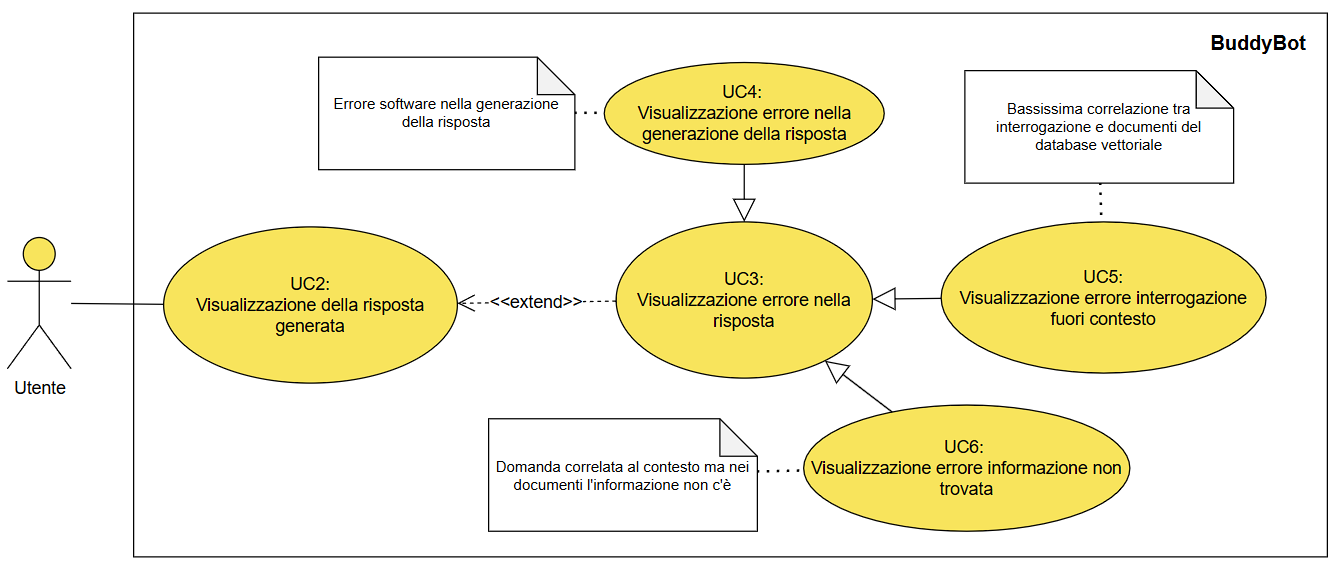
\includegraphics[width=\textwidth]{UC2+UC3+UC4+UC5+UC6.png}
    \caption{Visualizzazione della risposta generata}
\end{figure}

\begin{itemize}
    \item \textbf{Attori principali}: Utente;
    \item \textbf{Precondizioni}: Il sistema ha generato correttamente la risposta alla domanda dell'utente;
    \item \textbf{Trigger}: L'utente desidera visualizzare la risposta alla domanda che ha posto;
    \item \textbf{Postcondizioni}: L'utente visualizza la risposta generata dal sistema;
    \item \textbf{Scenario principale}:
    \begin{enumerate}
        \item Il sistema ha generato correttamente la risposta alla domanda dell'utente;
        \item L'utente visualizza la risposta generata dal sistema.
    \end{enumerate}
    \item \textbf{Scenario alternativo}:
    \begin{enumerate}
        \item \bulhyperlink{UC3}{UC3}: Visualizzazione errore nella risposta.
    \end{enumerate}
\end{itemize}

\hypertarget{UC3}{}
\subsubsection{UC3: Visualizzazione errore nella risposta}
\begin{itemize}
    \item \textbf{Attori principali}: Utente;
    \item \textbf{Precondizioni}: Il sistema non ha generato correttamente la risposta alla domanda dell'utente;
    \item \textbf{Trigger}: L'utente desidera visualizzare la risposta alla domanda che ha posto;
    \item \textbf{Postcondizioni}: Viene visualizzato un messaggio di errore;
    \item \textbf{Scenario principale}:
    \begin{enumerate}
        \item Il sistema ha generato correttamente la risposta alla domanda dell'utente;
        \item Avviene un errore (di qualunque tipo) durante il processo di generazione della risposta;
        \item Viene visualizzato un messaggio di errore.
    \end{enumerate}
    \item \textbf{Casi che ereditano}:
    \begin{itemize}
        \item \bulhyperlink{UC4}{UC4}: Visualizzazione errore nella generazione della risposta;
        \item \bulhyperlink{UC5}{UC5}: Visualizzazione errore interrogazione fuori contesto;
        \item \bulhyperlink{UC6}{UC6}: Visualizzazione errore informazione non trovata.
    \end{itemize}
\end{itemize}

\hypertarget{UC4}{}
\subsubsection{UC4: Visualizzazione errore nella generazione della risposta}
\begin{itemize}
    \item \textbf{Attori principali}: Utente;
    \item \textbf{Precondizioni}: Il sistema non è riuscito a generare la risposta alla domanda dell'utente a causa di un errore interno;
    \item \textbf{Trigger}: L'utente desidera ricevere una risposta in linguaggio naturale alla domanda che ha posto;
    \item \textbf{Postcondizioni}: Viene visualizzato un messaggio di errore, chiedendo di riprovare più tardi;
    \item \textbf{Scenario principale}:
    \begin{enumerate}
        \item \bulhyperlink{UC1}{UC1}: L'utente inserisce un'interrogazione in linguaggio naturale;
        \item Si genera un errore durante il processamento della domanda che non permette la generazione della risposta;
        \item Viene visualizzato un messaggio di errore, chiedendo di riprovare più tardi.
    \end{enumerate}
    \item \textbf{Eredita da}:
    \begin{itemize}
        \item \bulhyperlink{UC3}{UC3}: Visualizzazione errore nella risposta.
    \end{itemize}
\end{itemize}

\hypertarget{UC5}{}
\subsubsection{UC5: Visualizzazione errore interrogazione fuori contesto}
\begin{itemize}
    \item \textbf{Attori principali}: Utente;
    \item \textbf{Precondizioni}: Il sistema ha rilevato una bassissima correlazione tra l'interrogazione scritta dall'utente e i documenti del \emph{database vettoriale};
    \item \textbf{Trigger}: L'utente desidera visualizzare una risposta contenente informazioni legate esclusivamente ai contenuti del \emph{database vettoriale} associato al sistema;
    \item \textbf{Postcondizioni}: Viene visualizzato un messaggio che comunica all'utente che la domanda inserita è fuori contesto e che quindi è impossibile generare una risposta;
    \item \textbf{Scenario principale}:
    \begin{enumerate}
        \item \bulhyperlink{UC1}{UC1}: L'utente inserisce un'interrogazione in linguaggio naturale;
        \item Il sistema analizza la frase e cerca di contestualizzarla confrontandola con i dati presenti nel database;
        \item Il sistema rileva che la frase è fuori contesto e non può essere associata a nessuna informazione rilevante nel database;
        \item Il sistema invia un messaggio all'utente indicando che la domanda inserita è fuori contesto e richiede ulteriori chiarimenti.
    \end{enumerate}
    \item \textbf{Eredita da}:
    \begin{itemize}
        \item \bulhyperlink{UC3}{UC3}: Visualizzazione errore nella risposta.
    \end{itemize}
\end{itemize}

\hypertarget{UC6}{}
\subsubsection{UC6: Visualizzazione errore informazione non trovata}
\begin{itemize}
    \item \textbf{Attori coinvolti}: Utente;
    \item \textbf{Precondizioni}: Il sistema non ha trovato nei documenti di contesto l'informazione che l'utente ha domandato;
    \item \textbf{Trigger}: L'utente desidera visualizzare una risposta contenente le informazioni che ha richiesto nella domanda che ha posto al sistema;
    \item \textbf{Postcondizioni}: L'utente visualizza come risposta un messaggio del sistema in cui gli viene segnalata la mancanza dell'informazione 
    richiesta nei documenti individuati come contesto;
    \item \textbf{Scenario principale}:
    \begin{enumerate}
        \item Il sistema individua alcuni documenti di contesto nel \emph{database vettoriale} correlati alla domanda dell'utente;
        \item Il sistema non trova nei documenti di contesto l'informazione che l'utente ha domandato;
        \item L'utente visualizza come risposta un messaggio del sistema in cui gli viene segnalata la mancanza dell'informazione richiesta 
        nei documenti individuati come contesto.
    \end{enumerate}
    \item \textbf{Eredita da}:
    \begin{itemize}
        \item \bulhyperlink{UC3}{UC3}: Visualizzazione errore nella risposta.
    \end{itemize}
\end{itemize}


\hypertarget{UC2.1}{}
\subsubsubsection{UC2.1: Visualizzazione dei file da cui il sistema ha preso i dati per la risposta alla domanda}

\begin{figure}[h]
    \centering
    
\includegraphics[width=\textwidth]{placeholder.png}
    \caption{Visualizzazione dei file da cui il sistema ha preso i dati per la risposta alla domanda}
\end{figure}

\begin{itemize}
    \item \textbf{Attori principali}: Utente;
    \item \textbf{Precondizioni}: L'utente ha visualizzato la risposta generata con dati di contesto provenienti da \emph{GitHub}, \emph{Jira} e \emph{Confluence};
    \item \textbf{Trigger}: L'utente desidera visualizzare i file da cui il sistema ha preso i dati per la risposta alla domanda;
    \item \textbf{Postcondizioni}: L'utente visualizza i file da cui il sistema ha preso i dati per la risposta alla domanda;
    \item \textbf{Scenario principale}:
    \begin{enumerate}
        \item L'utente accede all'interfaccia dell'applicazione.
        \item \bulhyperlink{UC1}{UC1}: Inserimento di interrogazione in linguaggio naturale.
        \item \bulhyperlink{UC8}{UC8}: Visualizzare una risposta generata con dati di contesto provenienti da \emph{GitHub}, \emph{Jira} e \emph{Confluence}.
        \item Visualizzazione dei file da cui il sistema ha preso i dati per la risposta alla domanda.
    \end{enumerate}
    \item \textbf{Sottocasi d'uso}:
    \begin{itemize}
        \item \bulhyperlink{UC13.1}{UC13.1}: Il sistema recupera il nome e il percorso del file preso per elaborare la risposta;
        \item \bulhyperlink{UC13.2}{UC13.2}: Il sistema recupera il contesto specifico in cui ogni file è stato utilizzato
        per generare la risposta (es. paragrafo, frase, o parte di codice).
    \end{itemize}
    \item \textbf{Scenario alternativo}:
    \begin{enumerate}
        \item \bulhyperlink{UC18}{UC18}: Errore nella rilevazione dei file utili per la risposta.
    \end{enumerate}
\end{itemize}

\hypertarget{UC15}{}
\subsubsection{UC15: Visualizzazione errore nella rilevazione dei file utili per la risposta}
\begin{itemize}
    \item \textbf{Attori principali}: Utente;
    \item \textbf{Precondizioni}: L'utente ha visualizzato la risposta generata con dati di contesto provenienti da \emph{GitHub}, \emph{Jira} e \emph{Confluence};
    \item \textbf{Trigger}: L'utente desidera visualizzare i file da cui il sistema ha preso i dati per la risposta alla domanda;
    \item \textbf{Postcondizioni}: Viene visualizzato un messaggio di errore riferendo non è stato possibile rilevare i file da cui è stata ricavata la risposta;
    \item \textbf{Scenario principale}: 
    \begin{enumerate}
        \item L'utente accede all'interfaccia dell'applicazione;
        \item \bulhyperlink{UC1}{UC1}: Inserimento di interrogazione in linguaggio naturale;
        \item \bulhyperlink{UC8}{UC8}: Visualizzazione di una risposta generata con dati di contesto provenienti da \emph{GitHub}, \emph{Jira} e \emph{Confluence};
        \item Il sistema non riesce a rilevare i file da cui ha generato la risposta;
        \item L'utente visualizzera un messaggio di errore che comunica l'impossibilità di rilevare i file da cui è stata ricavata la risposta.
    \end{enumerate}
\end{itemize}


\hypertarget{UC7}{}
\subsubsection{UC7: Copia del testo della risposta generata}

\begin{figure}[h]
    \centering
    
\includegraphics[width=\textwidth]{placeholder.png}
    \caption{Copia del testo della risposta generata}
\end{figure}

\begin{itemize}
    \item \textbf{Attori principali}: Utente;
    \item \textbf{Precondizioni}: Il sistema ha generato una risposta valida e visibile alla domanda posta dall'utente;
    \item \textbf{Trigger}: L'utente desidera copiare il testo della risposta generata;
    \item \textbf{Postcondizioni}: Il testo della risposta generata viene copiato con successo nella clipboard del dispositivo e diventa disponibile per l'uso da parte dell'utente in altre applicazioni o contesti;
    \item \textbf{Scenario principale}:
    \begin{enumerate}
        \item \bulhyperlink{UC3}{UC3}: Il sistema ha generato correttamente la risposta alla domanda dell'utente;
        \item L'utente copia il testo della risposta generata;
    \end{enumerate}

    \item \textbf{Sottocasi d'uso}:
    \begin{itemize}
        \item \bulhyperlink{UC7.1}{UC7.1}: Copiare lo \emph{snippet} di codice inserito nella risposta;
    \end{itemize}
\end{itemize}


\hypertarget{UC8}{}
\subsubsubsection{UC8: Copia dello \emph{snippet} di codice inserito nella risposta}

\begin{figure}[h]
    \centering
    
\includegraphics[width=\textwidth]{placeholder.png}
    \caption{Copia dello \emph{snippet} di codice inserito nella risposta}
\end{figure}

\begin{itemize}
    \item \textbf{Attori principali}: Utente;
    \item \textbf{Precondizioni}: Il sistema ha generato una risposta valida con uno \emph{snippet} di codice al suo interno;
    \item \textbf{Trigger}:L'utente desidera copiare lo \emph{snippet} di codice inserito nella risposta;
    \item \textbf{Postcondizioni}: Lo \emph{snippet} di codice generato viene copiato con successo nella clipboard del dispositivo e diventa disponibile per l'uso da parte dell'utente in altre applicazioni o contesti;
    \item \textbf{Scenario principale}:
    \begin{enumerate}
        \item \bulhyperlink{UC3}{UC3}: Il sistema ha generato correttamente la risposta alla domanda dell'utente con al suo interno dello \emph{snippet} di codice;
        \item L'utente copia lo \emph{snippet} di codice;
    \end{enumerate}
\end{itemize}


\newpage
\hypertarget{UC9}{}
\subsubsection{UC9: Visualizzazione dello storico di sessione}

\begin{figure}[h]
    \centering
    
\includegraphics[width=\textwidth]{placeholder.png}
    \caption{Visualizzazione dello storico di sessione}
\end{figure}

\begin{itemize}
    \item \textbf{Attori principali}: Utente;
    \item \textbf{Precondizioni}: Il sistema deve essere collegato a un database relazionale per memorizzare e recuperare lo storico delle sessioni;
    \item \textbf{Trigger}: L'utente desidera visualizzare lo storico di sessione;
    \item \textbf{Postcondizioni}: L'utente visualizza lo storico di sessione;
    \item \textbf{Scenario principale}:
    \begin{enumerate}
        \item L'utente desidera recuperare lo storico di sessione;
        \item \bulhyperlink{UC9.1}{UC9.1}: Il sistema recupera i dati dello storico di sessione dal database relazionale e lo mostra a schermo;
        \item L'utente visualizza lo storico di sessione.
    \end{enumerate}

    \item \textbf{Sottocasi d'uso}:
    \begin{itemize}
        \item \bulhyperlink{UC9.1}{UC9.1}: Recupero dati dal database relazionale;
    \end{itemize}
    \item \textbf{Scenario alternativo}:
    \begin{enumerate}
        \item \bulhyperlink{UC17}{UC17}: Errore nel recupero dello storico.
    \end{enumerate}
\end{itemize}

\hypertarget{UC10}{}
\subsubsection{UC10: Visualizzazione errore nel recupero dello storico}
\begin{itemize}
    \item \textbf{Attori principali}: Utente;
    \item \textbf{Precondizioni}: L'utente ha richiesto di recuperare lo storico di sessione;
    \item \textbf{Trigger}: L'utente desidera visualizzare i dati dello storico di sessione;
    \item \textbf{Postcondizioni}: Viene visualizzato un messaggio di errore riferendo che c'è stato un errore nel recupero dello storico di sessione;
    \item \textbf{Scenario principale}: 
    \begin{enumerate}
        \item L'utente ha richiesto di recuperare lo storico di sessione memorizzato nel database relazionale;
        \item Il sistema ha riscontrato un problema e visualizza un messaggio di errore riferendo che c'è stato un errore nel recupero dello storico di sessione;
    \end{enumerate}
\end{itemize}


\hypertarget{UC11}{}
\subsubsection{UC11: Aggiornamento automatico del database vettoriale}

\begin{figure}[h]
    \centering
    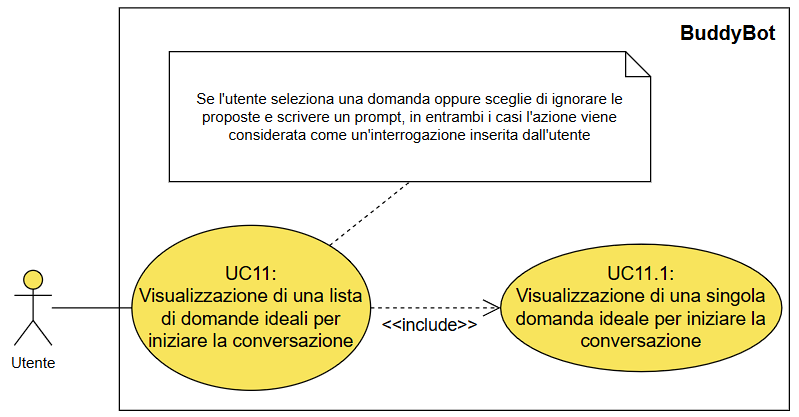
\includegraphics[width=\textwidth]{UC11.png}
    \caption{Aggiornamento automatico del database vettoriale}
\end{figure}

\begin{itemize}
    \item \textbf{Attori principali}: Scheduler;
    \item \textbf{Precondizioni}: 
    \begin{itemize}
        \item L'utente avvia l'applicazione;
        \item Il sistema è connesso al database vettoriale;
        \item Lo \emph{Scheduler} è attivo;
        \item E' arrivato il momento, prefissato dallo Scheduler, di aggiornare il database vettoriale.
    \end{itemize}
    \item \textbf{Trigger}: L'utente desidera ricevere risposte basate su dati aggiornati provenienti da GitHub, Jira e Confluence;
    \item \textbf{Postcondizioni}: Lo scheduler ha aggiornato il database vettoriale con i dati più recenti provenienti da GitHub, Jira e Confluence;
    \item \textbf{Scenario principale}:
    \begin{enumerate}
        \item E' arrivato il momento, prefissato dallo Scheduler, di aggiornare il database vettoriale;
        \item \bulhyperlink{UC11.1}{UC11.1}: Chiamata \emph{API}\textsubscript{\textbf{\textit{G}}} verso GitHub per il recupero di eventuali nuove modifiche;
        \item \bulhyperlink{UC11.2}{UC11.2}: Chiamata API verso Jira per il recupero di eventuali nuove modifiche;
        \item \bulhyperlink{UC11.3}{UC11.3}: Chiamata API verso Confluence per il recupero di eventuali nuove modifiche;
        \item \bulhyperlink{UC11.4.1}{UC11.4.1}: Conversione dei nuovi dati in formato vettoriale da parte del modello di embedding;
        \item \bulhyperlink{UC11.4}{UC11.4}: \emph{Merge}\textsubscript{\textbf{\textit{G}}} dei nuovi dati aggiornati di GitHub, Jira e Confluence
        con i dati già presenti nel database vettoriale.
    \end{enumerate}
    \item \textbf{Sottocasi d'uso}:
    \begin{itemize}
        \item \bulhyperlink{UC11.1}{UC11.1}: Chiamata API verso GitHub per il recupero di eventuali nuove modifiche;
        \item \bulhyperlink{UC11.2}{UC11.2}: Chiamata API verso Jira per il recupero di eventuali nuove modifiche;
        \item \bulhyperlink{UC11.3}{UC11.3}: Chiamata API verso Confluence per il recupero di eventuali nuove modifiche;
        \item \bulhyperlink{UC11.4}{UC11.4}: Merge delle risposte generate utilizzando dati di contesto di GitHub, Jira e Confluence aggiornati.
    \end{itemize}
\end{itemize}

\hypertarget{UC11.1}{}
\subsubsubsection{UC11.1: Chiamata API verso GitHub per il recupero di eventuali nuove modifiche}
\begin{itemize}
    \item \textbf{Attori principali}: GitHub;
    \item \textbf{Precondizioni}: E' arrivato il momento, prefissato dallo Scheduler, di aggiornare il database vettoriale;
    \item \textbf{Trigger}: L'utente desidera ricevere risposte basate su dati aggiornati provenienti da GitHub;
    \item \textbf{Postcondizioni}: Vengono recuperati i dati aggiornati da GitHub;
    \item \textbf{Scenario principale}: 
    \begin{enumerate}
        \item E' arrivato il momento, prefissato dallo Scheduler, di aggiornare il database vettoriale;
        \item Avviene una chiamata API verso GitHub per il recupero dei dati più recenti;
        \item Vengono recuperati i dati aggiornati da GitHub.
    \end{enumerate}
\end{itemize}

\hypertarget{UC11.2}{}
\subsubsubsection{UC11.2: Chiamata API verso Jira per il recupero di eventuali nuove modifiche}
\begin{itemize}
    \item \textbf{Attori principali}: Jira;
    \item \textbf{Precondizioni}: E' arrivato il momento, prefissato dallo Scheduler, di aggiornare il database vettoriale;
    \item \textbf{Trigger}: L'utente desidera ricevere risposte basate su dati aggiornati provenienti da Jira;
    \item \textbf{Postcondizioni}: Vengono recuperati i dati aggiornati da Jira;
    \item \textbf{Scenario principale}: 
    \begin{enumerate}
        \item E' arrivato il momento, prefissato dallo Scheduler, di aggiornare il database vettoriale;
        \item Avviene una chiamata API verso Jira per il recupero dei dati più recenti;
        \item Vengono recuperati i dati aggiornati da Jira.
    \end{enumerate}
\end{itemize}

\hypertarget{UC11.3}{}
\subsubsubsection{UC11.3: Chiamata API verso Confluence per il recupero di eventuali nuove modifiche}
\begin{itemize}
    \item \textbf{Attori principali}: Confluence;
    \item \textbf{Precondizioni}: E' arrivato il momento, prefissato dallo Scheduler, di aggiornare il database vettoriale;
    \item \textbf{Trigger}: L'utente desidera ricevere risposte basate su dati aggiornati provenienti da Confluence;
    \item \textbf{Postcondizioni}: Vengono recuperati i dati aggiornati da Confluence;
    \item \textbf{Scenario principale}: 
    \begin{enumerate}
        \item E' arrivato il momento, prefissato dallo Scheduler, di aggiornare il database vettoriale;
        \item Avviene una chiamata API verso Confluence per il recupero dei dati più recenti;
        \item Vengono recuperati i dati aggiornati da Confluence.
    \end{enumerate}
\end{itemize}

\hypertarget{UC11.4}{}
\subsubsubsection{UC11.4: Merge dei nuovi dati con i dati già presenti nel database vettoriale}
\begin{itemize}
    \item \textbf{Attori principali}: Database vettoriale;
    \item \textbf{Precondizioni}: Sono stati recuperati i dati aggiornati da GitHub, Jira e Confluence;
    \item \textbf{Trigger}: L'utente desidera ricevere risposte basate su dati aggiornati provenienti da GitHub, Jira e Confluence;
    \item \textbf{Postcondizioni}: E' stato eseguito il merge dei nuovi dati provenienti da GitHub, Jira e Confluence nel database vettoriale;
    \item \textbf{Scenario principale}:
    \begin{enumerate}
        \item E' arrivato il momento, prefissato dallo Scheduler, di aggiornare il database vettoriale;
        \item \bulhyperlink{UC11.1}{UC11.1}: Chiamata API verso GitHub per il recupero di eventuali nuove modifiche;
        \item \bulhyperlink{UC11.2}{UC11.2}: Chiamata API verso Jira per il recupero di eventuali nuove modifiche;
        \item \bulhyperlink{UC11.3}{UC11.3}: Chiamata API verso Confluence per il recupero di eventuali nuove modifiche;
        \item \bulhyperlink{UC11.4.1}{UC11.4.1}: I nuovi dati provenienti da GitHub, Jira e Confluence vengono convertiti in formato vettoriale dal modello di embedding;
        \item Viene eseguito il merge dei nuovi dati in formato vettoriale con i dati già presenti nel database vettoriale.
    \end{enumerate}
    \item \textbf{Sottocasi d'uso}:
    \begin{itemize}
        \item \bulhyperlink{UC11.4.1}{UC11.4.1}: Conversione dei nuovi dati in formato vettoriale.
    \end{itemize}
\end{itemize}

\hypertarget{UC11.4.1}{}
\paragraph{UC11.4.1: Conversione dei nuovi dati in formato vettoriale}
\begin{itemize}
    \item \textbf{Attori principali}: Modello di embedding;
    \item \textbf{Precondizioni}: Sono stati recuperati i dati aggiornati da GitHub, Jira e Confluence;
    \item \textbf{Trigger}: L'utente desidera ricevere risposte basate su dati aggiornati provenienti da GitHub, Jira e Confluence;
    \item \textbf{Postcondizioni}: I nuovi dati provenienti da GitHub, Jira e Confluence vengono convertiti in formato vettoriale dal modello di embedding;
    \item \textbf{Scenario principale}: 
    \begin{enumerate}
        \item E' arrivato il momento, prefissato dallo Scheduler, di aggiornare il database vettoriale;
        \item \bulhyperlink{UC11.1}{UC11.1}: Chiamata API verso GitHub per il recupero di eventuali nuove modifiche;
        \item \bulhyperlink{UC11.2}{UC11.2}: Chiamata API verso Jira per il recupero di eventuali nuove modifiche;
        \item \bulhyperlink{UC11.3}{UC11.3}: Chiamata API verso Confluence per il recupero di eventuali nuove modifiche;
        \item I nuovi dati provenienti da GitHub, Jira e Confluence vengono convertiti in formato vettoriale dal modello di embedding.
    \end{enumerate}
\end{itemize}


\hypertarget{UC12}{}
\subsubsection{UC12: Visualizzazione di una lista di domande ideali per iniziare la conversazione}

\begin{figure}[h]
    \centering
    
\includegraphics[width=\textwidth]{placeholder.png}
    \caption{Visualizzazione di una lista di domande ideali per iniziare la conversazione}
\end{figure}

\begin{itemize}
    \item \textbf{Attori principali}: Utente;
    \item \textbf{Precondizioni}: L'utente ha appena cominciato una nuova conversazione;
    \item \textbf{Trigger}: L'utente desidera ricevere delle proposte di possibili domande per iniziare la conversazione;
    \item \textbf{Postcondizioni}: L'utente ha ricevuto una serie di domande suggerite dal sistema, che possono essere utilizzate per iniziare la conversazione;
    \item \textbf{Scenario principale}:
    \begin{enumerate}
        \item L'utente avvia l'applicazione;
        \item Il sistema propone una lista di domande ideali per iniziare la conversazione;
        \item L'utente seleziona una delle domande proposte o inserisce una propria domanda.
    \end{enumerate}
    \item \textbf{Sottocasi d'uso}:
    \begin{itemize}
        \item \bulhyperlink{UC12.1}{UC12.1}: Visualizzare una singola domanda ideale per iniziare la conversazione;
    \end{itemize}
\end{itemize}

\hypertarget{UC12.1}{}
\subsubsection{UC12.1: Visualizzazione di una singola domanda ideale per iniziare la conversazione}
\begin{itemize}
    \item \textbf{Attori principali}: Utente;
    \item \textbf{Precondizioni}: L'utente ha appena cominciato una nuova conversazione;
    \item \textbf{Trigger}: L'utente desidera ricevere una proposta di domanda per iniziare la conversazione;
    \item \textbf{Postcondizioni}: L'utente visualizza una domanda suggerita dal sistema, che può essere utilizzata per iniziare la conversazione;
    \item \textbf{Scenario principale}:
    \begin{enumerate}
        \item L'utente avvia l'applicazione;
        \item Il sistema propone una domanda ideale;
        \item \bulhyperlink{UC1}{UC1}: L'utente seleziona la domanda proposta o inserisce una propria domanda.
    \end{enumerate}
\end{itemize}


\hypertarget{UC13}{}
\subsubsection{UC13: Visualizzazione di una lista di domande ideali per proseguire la conversazione}

\begin{figure}[h]
    \centering
    
\includegraphics[width=\textwidth]{placeholder.png}
    \caption{Visualizzazione di una lista di domande ideali per proseguire la conversazione}
\end{figure}

\begin{itemize}
    \item \textbf{Attori principali}: Utente;
    \item \textbf{Precondizioni}: L'utente ha appena ricevuto una risposta dal sistema;
    \item \textbf{Trigger}: L'utente desidera ricevere delle proposte di possibili domande per proseguire la conversazione;
    \item \textbf{Postcondizioni}: L'utente ha ricevuto una lista di domande suggerite dal sistema, che possono essere utilizzate per proseguire la conversazione;
    \item \textbf{Scenario principale}:
    \begin{enumerate}
        \item \bulhyperlink{UC5}{UC5}: L'utente ha visualizzato la risposta a una domanda precedente;
        \item Il sistema propone una lista di domande considerate utili rispetto ai messaggi precedenti;
        \item \bulhyperlink{UC1}{UC1}: L'utente seleziona una delle domande proposte o inserisce una propria domanda;
    \end{enumerate}
    \item \textbf{Sottocasi d'uso}:
    \begin{itemize}
        \item \bulhyperlink{UC14.1}{UC14.1}: Visualizzare una singola domanda ideale per proseguire la conversazione.
    \end{itemize}
    \item \textbf{Scenario alternativo}:
    \begin{enumerate}
        \item \bulhyperlink{UC15}{UC15}: Visualizzazione di un messaggio di errore che comunica che il sistema non è in grado di proporre delle domande.
    \end{enumerate}
\end{itemize}

\hypertarget{UC13.1}{}
\subsubsection{UC13.1: Visualizzazione di una singola domanda ideale per proseguire la conversazione}
\begin{itemize}
    \item \textbf{Attori principali}: Utente;
    \item \textbf{Precondizioni}: L'utente ha appena ricevuto una risposta dal sistema;
    \item \textbf{Trigger}: L'utente desidera ricevere una proposta di domanda per proseguire la conversazione;
    \item \textbf{Postcondizioni}: L'utente visualizza una domanda suggerita dal sistema, che può essere utilizzata per proseguire la conversazione;
    \item \textbf{Scenario principale}:
    \begin{enumerate}
        \item \bulhyperlink{UC5}{UC5}: L'utente ha visualizzato la risposta a una domanda precedente;
        \item Il sistema propone una domanda ideale per proseguire la conversazione;
        \item \bulhyperlink{UC1}{UC1}: L'utente seleziona la domanda proposta o inserisce una propria domanda;
    \end{enumerate}
\end{itemize}

\hypertarget{UC14}{}
\subsubsection{UC14: Visualizzazione errore nella generazione delle domande per proseguire la conversazione}
\begin{itemize}
    \item \textbf{Attori principali}: Utente;
    \item \textbf{Precondizioni}: L'utente ha appena ricevuto una risposta dal sistema;
    \item \textbf{Trigger}: L'utente desidera ricevere delle proposte di possibili domande per proseguire la conversazione;
    \item \textbf{Postcondizioni}: L'utente ha ricevuto un messaggio di errore che comunica che il sistema non è in grado di proporre delle domande;
    \item \textbf{Scenario principale}:
    \begin{enumerate}
        \item \bulhyperlink{UC5}{UC5}: L'utente ha visualizzato la risposta a una domanda precedente;
        \item Il sistema mostra un messaggio di errore che comunica che non è in grado di proporre delle domande.
    \end{enumerate}
\end{itemize}


\hypertarget{UC16}{}
\subsubsection{UC16: Visualizzazione dei log di aggiornamento del database vettoriale}

\begin{figure}[h]
    \centering
    
\includegraphics[width=\textwidth]{placeholder.png}
    \caption{Visualizzazione dei log di aggiornamento del database vettoriale}
\end{figure}

\dots

\hypertarget{UC17}{}
\subsubsection{UC17: Visualizzazione errore nel recupero dei log di aggiornamento del database vettoriale}
\dots

\newpage

\hypertarget{UC18}{}
\subsubsection{UC18: Visualizzazione di un badge che segnala lo stato di aggiornamento del database vettoriale}

\begin{figure}[h]
    \centering
    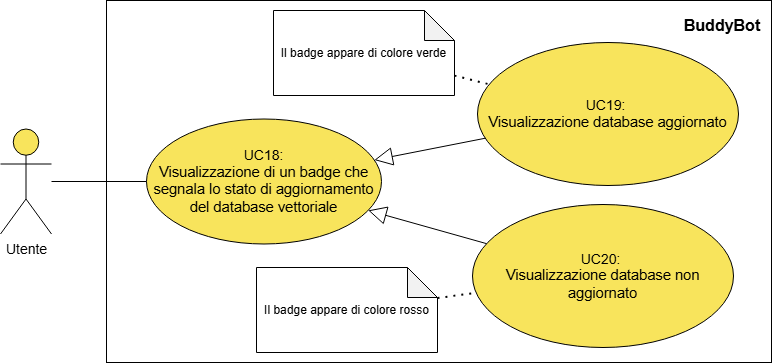
\includegraphics[width=\textwidth]{UC18+UC19+UC20.png}
    \caption{Visualizzazione di un badge che segnala lo stato di aggiornamento del database vettoriale}
\end{figure}

\begin{itemize}
    \item \textbf{Attori principali}: Utente;
    \item \textbf{Precondizioni}: L'utente avvia l'applicazione;
    \item \textbf{Trigger}: L'utente desidera verificare se il database vettoriale è stato aggiornato;
    \item \textbf{Postcondizioni}: L'utente visualizza un badge che segnala lo stato di aggiornamento del database vettoriale;
    \item \textbf{Scenario principale}:
    \begin{enumerate}
        \item L'utente avvia l'applicazione;
        \item Il sistema segnala lo stato di aggiornamento del database vettoriale;
    \end{enumerate}
    \item \textbf{Casi che ereditano}:
    \begin{itemize}
        \item \bulhyperlink{UC19}{UC19}: Visualizzazione database aggiornato;
        \item \bulhyperlink{UC20}{UC20}: Visualizzazione database non aggiornato;
    \end{itemize}
\end{itemize}

\hypertarget{UC19}{}
\subsubsection{UC19: Visualizzazione database aggiornato}
\begin{itemize}
    \item \textbf{Attori principali}: Utente;
    \item \textbf{Precondizioni}: L'utente avvia l'applicazione;
    \item \textbf{Trigger}: L'utente desidera verificare se il database vettoriale è stato aggiornato;
    \item \textbf{Postcondizioni}: L'utente visualizza un badge indicativo che il database vettoriale è aggiornato;
    \item \textbf{Scenario principale}:
    \begin{enumerate}
        \item L'utente avvia l'applicazione;
        \item Il sistema segnala che il database vettoriale è aggiornato tramite un badge di colore verde;
    \end{enumerate}
    \item \textbf{Eredita da}:
    \begin{itemize}
        \item \bulhyperlink{UC18}{UC18}: Visualizzazione di un badge che segnala lo stato di aggiornamento del database vettoriale;
    \end{itemize}
\end{itemize}

\hypertarget{UC20}{}
\subsubsection{UC20: Visualizzazione database non aggiornato}
\begin{itemize}
    \item \textbf{Attori principali}: Utente;
    \item \textbf{Precondizioni}: L'utente avvia l'applicazione;
    \item \textbf{Trigger}: L'utente desidera verificare se il database vettoriale è stato aggiornato;
    \item \textbf{Postcondizioni}: L'utente visualizza un badge indicativo che il database vettoriale non è aggiornato;
    \item \textbf{Scenario principale}:
    \begin{enumerate}
        \item L'utente avvia l'applicazione;
        \item Il sistema segnala che il database vettoriale non è aggiornato tramite un badge di colore rosso;
    \end{enumerate}
    \item \textbf{Eredita da}:
    \begin{itemize}
        \item \bulhyperlink{UC18}{UC18}: Visualizzazione di un badge che segnala lo stato di aggiornamento del database vettoriale;
    \end{itemize}
\end{itemize}

